% GNUPLOT: LaTeX picture with Postscript
\begingroup
  \makeatletter
  \providecommand\color[2][]{%
    \GenericError{(gnuplot) \space\space\space\@spaces}{%
      Package color not loaded in conjunction with
      terminal option `colourtext'%
    }{See the gnuplot documentation for explanation.%
    }{Either use 'blacktext' in gnuplot or load the package
      color.sty in LaTeX.}%
    \renewcommand\color[2][]{}%
  }%
  \providecommand\includegraphics[2][]{%
    \GenericError{(gnuplot) \space\space\space\@spaces}{%
      Package graphicx or graphics not loaded%
    }{See the gnuplot documentation for explanation.%
    }{The gnuplot epslatex terminal needs graphicx.sty or graphics.sty.}%
    \renewcommand\includegraphics[2][]{}%
  }%
  \providecommand\rotatebox[2]{#2}%
  \@ifundefined{ifGPcolor}{%
    \newif\ifGPcolor
    \GPcolortrue
  }{}%
  \@ifundefined{ifGPblacktext}{%
    \newif\ifGPblacktext
    \GPblacktexttrue
  }{}%
  % define a \g@addto@macro without @ in the name:
  \let\gplgaddtomacro\g@addto@macro
  % define empty templates for all commands taking text:
  \gdef\gplbacktext{}%
  \gdef\gplfronttext{}%
  \makeatother
  \ifGPblacktext
    % no textcolor at all
    \def\colorrgb#1{}%
    \def\colorgray#1{}%
  \else
    % gray or color?
    \ifGPcolor
      \def\colorrgb#1{\color[rgb]{#1}}%
      \def\colorgray#1{\color[gray]{#1}}%
      \expandafter\def\csname LTw\endcsname{\color{white}}%
      \expandafter\def\csname LTb\endcsname{\color{black}}%
      \expandafter\def\csname LTa\endcsname{\color{black}}%
      \expandafter\def\csname LT0\endcsname{\color[rgb]{1,0,0}}%
      \expandafter\def\csname LT1\endcsname{\color[rgb]{0,1,0}}%
      \expandafter\def\csname LT2\endcsname{\color[rgb]{0,0,1}}%
      \expandafter\def\csname LT3\endcsname{\color[rgb]{1,0,1}}%
      \expandafter\def\csname LT4\endcsname{\color[rgb]{0,1,1}}%
      \expandafter\def\csname LT5\endcsname{\color[rgb]{1,1,0}}%
      \expandafter\def\csname LT6\endcsname{\color[rgb]{0,0,0}}%
      \expandafter\def\csname LT7\endcsname{\color[rgb]{1,0.3,0}}%
      \expandafter\def\csname LT8\endcsname{\color[rgb]{0.5,0.5,0.5}}%
    \else
      % gray
      \def\colorrgb#1{\color{black}}%
      \def\colorgray#1{\color[gray]{#1}}%
      \expandafter\def\csname LTw\endcsname{\color{white}}%
      \expandafter\def\csname LTb\endcsname{\color{black}}%
      \expandafter\def\csname LTa\endcsname{\color{black}}%
      \expandafter\def\csname LT0\endcsname{\color{black}}%
      \expandafter\def\csname LT1\endcsname{\color{black}}%
      \expandafter\def\csname LT2\endcsname{\color{black}}%
      \expandafter\def\csname LT3\endcsname{\color{black}}%
      \expandafter\def\csname LT4\endcsname{\color{black}}%
      \expandafter\def\csname LT5\endcsname{\color{black}}%
      \expandafter\def\csname LT6\endcsname{\color{black}}%
      \expandafter\def\csname LT7\endcsname{\color{black}}%
      \expandafter\def\csname LT8\endcsname{\color{black}}%
    \fi
  \fi
    \setlength{\unitlength}{0.0500bp}%
    \ifx\gptboxheight\undefined%
      \newlength{\gptboxheight}%
      \newlength{\gptboxwidth}%
      \newsavebox{\gptboxtext}%
    \fi%
    \setlength{\fboxrule}{0.5pt}%
    \setlength{\fboxsep}{1pt}%
\begin{picture}(7920.00,7920.00)%
    \gplgaddtomacro\gplbacktext{%
      \csname LTb\endcsname%
      \put(957,5485){\makebox(0,0)[r]{\strut{}$10^{-3}$}}%
      \csname LTb\endcsname%
      \put(957,5803){\makebox(0,0)[r]{\strut{}$10^{-2}$}}%
      \csname LTb\endcsname%
      \put(957,6122){\makebox(0,0)[r]{\strut{}$10^{-1}$}}%
      \csname LTb\endcsname%
      \put(957,6440){\makebox(0,0)[r]{\strut{}$10^{0}$}}%
      \csname LTb\endcsname%
      \put(957,6759){\makebox(0,0)[r]{\strut{}$10^{1}$}}%
      \csname LTb\endcsname%
      \put(957,7077){\makebox(0,0)[r]{\strut{}$10^{2}$}}%
      \csname LTb\endcsname%
      \put(957,7396){\makebox(0,0)[r]{\strut{}$10^{3}$}}%
      \csname LTb\endcsname%
      \put(957,7714){\makebox(0,0)[r]{\strut{}$10^{4}$}}%
      \csname LTb\endcsname%
      \put(1059,5306){\makebox(0,0){\strut{} }}%
      \csname LTb\endcsname%
      \put(1335,5306){\makebox(0,0){\strut{} }}%
      \csname LTb\endcsname%
      \put(1611,5306){\makebox(0,0){\strut{} }}%
      \csname LTb\endcsname%
      \put(1886,5306){\makebox(0,0){\strut{} }}%
      \csname LTb\endcsname%
      \put(2162,5306){\makebox(0,0){\strut{} }}%
      \csname LTb\endcsname%
      \put(2438,5306){\makebox(0,0){\strut{} }}%
      \csname LTb\endcsname%
      \put(2714,5306){\makebox(0,0){\strut{} }}%
      \csname LTb\endcsname%
      \put(2990,5306){\makebox(0,0){\strut{} }}%
      \csname LTb\endcsname%
      \put(3265,5306){\makebox(0,0){\strut{} }}%
      \csname LTb\endcsname%
      \put(3541,5306){\makebox(0,0){\strut{} }}%
      \csname LTb\endcsname%
      \put(3817,5306){\makebox(0,0){\strut{} }}%
      \csname LTb\endcsname%
      \put(3919,5485){\makebox(0,0)[l]{\strut{} }}%
      \csname LTb\endcsname%
      \put(3919,5708){\makebox(0,0)[l]{\strut{} }}%
      \csname LTb\endcsname%
      \put(3919,5931){\makebox(0,0)[l]{\strut{} }}%
      \csname LTb\endcsname%
      \put(3919,6154){\makebox(0,0)[l]{\strut{} }}%
      \csname LTb\endcsname%
      \put(3919,6377){\makebox(0,0)[l]{\strut{} }}%
      \csname LTb\endcsname%
      \put(3919,6599){\makebox(0,0)[l]{\strut{} }}%
      \csname LTb\endcsname%
      \put(3919,6822){\makebox(0,0)[l]{\strut{} }}%
      \csname LTb\endcsname%
      \put(3919,7045){\makebox(0,0)[l]{\strut{} }}%
      \csname LTb\endcsname%
      \put(3919,7268){\makebox(0,0)[l]{\strut{} }}%
      \csname LTb\endcsname%
      \put(3919,7491){\makebox(0,0)[l]{\strut{} }}%
      \csname LTb\endcsname%
      \put(3919,7714){\makebox(0,0)[l]{\strut{} }}%
      \csname LTb\endcsname%
      \put(1059,7893){\makebox(0,0){\strut{}$10^{2}$}}%
      \csname LTb\endcsname%
      \put(1611,7893){\makebox(0,0){\strut{}$10^{3}$}}%
      \csname LTb\endcsname%
      \put(2162,7893){\makebox(0,0){\strut{}$10^{4}$}}%
      \csname LTb\endcsname%
      \put(2714,7893){\makebox(0,0){\strut{}$10^{5}$}}%
      \csname LTb\endcsname%
      \put(3265,7893){\makebox(0,0){\strut{}$10^{6}$}}%
      \csname LTb\endcsname%
      \put(3817,7893){\makebox(0,0){\strut{}$10^{7}$}}%
    }%
    \gplgaddtomacro\gplfronttext{%
      \csname LTb\endcsname%
      \put(357,6599){\rotatebox{-270}{\makebox(0,0){\strut{}$k = 2$}}}%
    }%
    \gplgaddtomacro\gplbacktext{%
      \csname LTb\endcsname%
      \put(3999,5485){\makebox(0,0)[r]{\strut{} }}%
      \csname LTb\endcsname%
      \put(3999,5708){\makebox(0,0)[r]{\strut{} }}%
      \csname LTb\endcsname%
      \put(3999,5931){\makebox(0,0)[r]{\strut{} }}%
      \csname LTb\endcsname%
      \put(3999,6154){\makebox(0,0)[r]{\strut{} }}%
      \csname LTb\endcsname%
      \put(3999,6377){\makebox(0,0)[r]{\strut{} }}%
      \csname LTb\endcsname%
      \put(3999,6599){\makebox(0,0)[r]{\strut{} }}%
      \csname LTb\endcsname%
      \put(3999,6822){\makebox(0,0)[r]{\strut{} }}%
      \csname LTb\endcsname%
      \put(3999,7045){\makebox(0,0)[r]{\strut{} }}%
      \csname LTb\endcsname%
      \put(3999,7268){\makebox(0,0)[r]{\strut{} }}%
      \csname LTb\endcsname%
      \put(3999,7491){\makebox(0,0)[r]{\strut{} }}%
      \csname LTb\endcsname%
      \put(3999,7714){\makebox(0,0)[r]{\strut{} }}%
      \csname LTb\endcsname%
      \put(4101,5306){\makebox(0,0){\strut{} }}%
      \csname LTb\endcsname%
      \put(4377,5306){\makebox(0,0){\strut{} }}%
      \csname LTb\endcsname%
      \put(4653,5306){\makebox(0,0){\strut{} }}%
      \csname LTb\endcsname%
      \put(4928,5306){\makebox(0,0){\strut{} }}%
      \csname LTb\endcsname%
      \put(5204,5306){\makebox(0,0){\strut{} }}%
      \csname LTb\endcsname%
      \put(5480,5306){\makebox(0,0){\strut{} }}%
      \csname LTb\endcsname%
      \put(5756,5306){\makebox(0,0){\strut{} }}%
      \csname LTb\endcsname%
      \put(6032,5306){\makebox(0,0){\strut{} }}%
      \csname LTb\endcsname%
      \put(6307,5306){\makebox(0,0){\strut{} }}%
      \csname LTb\endcsname%
      \put(6583,5306){\makebox(0,0){\strut{} }}%
      \csname LTb\endcsname%
      \put(6859,5306){\makebox(0,0){\strut{} }}%
      \csname LTb\endcsname%
      \put(6961,5485){\makebox(0,0)[l]{\strut{}$10^{-3}$}}%
      \csname LTb\endcsname%
      \put(6961,5803){\makebox(0,0)[l]{\strut{}$10^{-2}$}}%
      \csname LTb\endcsname%
      \put(6961,6122){\makebox(0,0)[l]{\strut{}$10^{-1}$}}%
      \csname LTb\endcsname%
      \put(6961,6440){\makebox(0,0)[l]{\strut{}$10^{0}$}}%
      \csname LTb\endcsname%
      \put(6961,6759){\makebox(0,0)[l]{\strut{}$10^{1}$}}%
      \csname LTb\endcsname%
      \put(6961,7077){\makebox(0,0)[l]{\strut{}$10^{2}$}}%
      \csname LTb\endcsname%
      \put(6961,7396){\makebox(0,0)[l]{\strut{}$10^{3}$}}%
      \csname LTb\endcsname%
      \put(6961,7714){\makebox(0,0)[l]{\strut{}$10^{4}$}}%
      \csname LTb\endcsname%
      \put(4101,7893){\makebox(0,0){\strut{}$10^{2}$}}%
      \csname LTb\endcsname%
      \put(4653,7893){\makebox(0,0){\strut{}$10^{3}$}}%
      \csname LTb\endcsname%
      \put(5204,7893){\makebox(0,0){\strut{}$10^{4}$}}%
      \csname LTb\endcsname%
      \put(5756,7893){\makebox(0,0){\strut{}$10^{5}$}}%
      \csname LTb\endcsname%
      \put(6307,7893){\makebox(0,0){\strut{}$10^{6}$}}%
      \csname LTb\endcsname%
      \put(6859,7893){\makebox(0,0){\strut{}$10^{7}$}}%
    }%
    \gplgaddtomacro\gplfronttext{%
      \csname LTb\endcsname%
      \put(7559,6599){\rotatebox{-270}{\makebox(0,0){\strut{}$k = 3$}}}%
    }%
    \gplgaddtomacro\gplbacktext{%
      \csname LTb\endcsname%
      \put(957,2845){\makebox(0,0)[r]{\strut{}$10^{-3}$}}%
      \csname LTb\endcsname%
      \put(957,3163){\makebox(0,0)[r]{\strut{}$10^{-2}$}}%
      \csname LTb\endcsname%
      \put(957,3482){\makebox(0,0)[r]{\strut{}$10^{-1}$}}%
      \csname LTb\endcsname%
      \put(957,3800){\makebox(0,0)[r]{\strut{}$10^{0}$}}%
      \csname LTb\endcsname%
      \put(957,4119){\makebox(0,0)[r]{\strut{}$10^{1}$}}%
      \csname LTb\endcsname%
      \put(957,4437){\makebox(0,0)[r]{\strut{}$10^{2}$}}%
      \csname LTb\endcsname%
      \put(957,4756){\makebox(0,0)[r]{\strut{}$10^{3}$}}%
      \csname LTb\endcsname%
      \put(957,5074){\makebox(0,0)[r]{\strut{}$10^{4}$}}%
      \csname LTb\endcsname%
      \put(1059,2666){\makebox(0,0){\strut{} }}%
      \csname LTb\endcsname%
      \put(1611,2666){\makebox(0,0){\strut{} }}%
      \csname LTb\endcsname%
      \put(2162,2666){\makebox(0,0){\strut{} }}%
      \csname LTb\endcsname%
      \put(2714,2666){\makebox(0,0){\strut{} }}%
      \csname LTb\endcsname%
      \put(3265,2666){\makebox(0,0){\strut{} }}%
      \csname LTb\endcsname%
      \put(3817,2666){\makebox(0,0){\strut{} }}%
      \csname LTb\endcsname%
      \put(3919,2845){\makebox(0,0)[l]{\strut{} }}%
      \csname LTb\endcsname%
      \put(3919,3068){\makebox(0,0)[l]{\strut{} }}%
      \csname LTb\endcsname%
      \put(3919,3291){\makebox(0,0)[l]{\strut{} }}%
      \csname LTb\endcsname%
      \put(3919,3514){\makebox(0,0)[l]{\strut{} }}%
      \csname LTb\endcsname%
      \put(3919,3737){\makebox(0,0)[l]{\strut{} }}%
      \csname LTb\endcsname%
      \put(3919,3959){\makebox(0,0)[l]{\strut{} }}%
      \csname LTb\endcsname%
      \put(3919,4182){\makebox(0,0)[l]{\strut{} }}%
      \csname LTb\endcsname%
      \put(3919,4405){\makebox(0,0)[l]{\strut{} }}%
      \csname LTb\endcsname%
      \put(3919,4628){\makebox(0,0)[l]{\strut{} }}%
      \csname LTb\endcsname%
      \put(3919,4851){\makebox(0,0)[l]{\strut{} }}%
      \csname LTb\endcsname%
      \put(3919,5074){\makebox(0,0)[l]{\strut{} }}%
      \csname LTb\endcsname%
      \put(1059,5253){\makebox(0,0){\strut{} }}%
      \csname LTb\endcsname%
      \put(1335,5253){\makebox(0,0){\strut{} }}%
      \csname LTb\endcsname%
      \put(1611,5253){\makebox(0,0){\strut{} }}%
      \csname LTb\endcsname%
      \put(1886,5253){\makebox(0,0){\strut{} }}%
      \csname LTb\endcsname%
      \put(2162,5253){\makebox(0,0){\strut{} }}%
      \csname LTb\endcsname%
      \put(2438,5253){\makebox(0,0){\strut{} }}%
      \csname LTb\endcsname%
      \put(2714,5253){\makebox(0,0){\strut{} }}%
      \csname LTb\endcsname%
      \put(2990,5253){\makebox(0,0){\strut{} }}%
      \csname LTb\endcsname%
      \put(3265,5253){\makebox(0,0){\strut{} }}%
      \csname LTb\endcsname%
      \put(3541,5253){\makebox(0,0){\strut{} }}%
      \csname LTb\endcsname%
      \put(3817,5253){\makebox(0,0){\strut{} }}%
    }%
    \gplgaddtomacro\gplfronttext{%
      \csname LTb\endcsname%
      \put(357,3959){\rotatebox{-270}{\makebox(0,0){\strut{}$k = 5$}}}%
      \csname LTb\endcsname%
      \put(5892,2118){\makebox(0,0)[r]{\strut{}Mult Gr w Blk Jac}}%
      \csname LTb\endcsname%
      \put(5892,1939){\makebox(0,0)[r]{\strut{}LAPACK}}%
      \csname LTb\endcsname%
      \put(5892,1760){\makebox(0,0)[r]{\strut{}Add Swz}}%
      \csname LTb\endcsname%
      \put(5892,1581){\makebox(0,0)[r]{\strut{}Pardiso w Blk PC}}%
      \csname LTb\endcsname%
      \put(5892,1402){\makebox(0,0)[r]{\strut{}Add Swz w Coarse}}%
      \csname LTb\endcsname%
      \put(5892,1223){\makebox(0,0)[r]{\strut{}Mumps}}%
      \csname LTb\endcsname%
      \put(5892,1044){\makebox(0,0)[r]{\strut{}Pardiso}}%
      \csname LTb\endcsname%
      \put(5892,865){\makebox(0,0)[r]{\strut{}linear}}%
    }%
    \gplgaddtomacro\gplbacktext{%
      \csname LTb\endcsname%
      \put(3999,2845){\makebox(0,0)[r]{\strut{} }}%
      \csname LTb\endcsname%
      \put(3999,3068){\makebox(0,0)[r]{\strut{} }}%
      \csname LTb\endcsname%
      \put(3999,3291){\makebox(0,0)[r]{\strut{} }}%
      \csname LTb\endcsname%
      \put(3999,3514){\makebox(0,0)[r]{\strut{} }}%
      \csname LTb\endcsname%
      \put(3999,3737){\makebox(0,0)[r]{\strut{} }}%
      \csname LTb\endcsname%
      \put(3999,3959){\makebox(0,0)[r]{\strut{} }}%
      \csname LTb\endcsname%
      \put(3999,4182){\makebox(0,0)[r]{\strut{} }}%
      \csname LTb\endcsname%
      \put(3999,4405){\makebox(0,0)[r]{\strut{} }}%
      \csname LTb\endcsname%
      \put(3999,4628){\makebox(0,0)[r]{\strut{} }}%
      \csname LTb\endcsname%
      \put(3999,4851){\makebox(0,0)[r]{\strut{} }}%
      \csname LTb\endcsname%
      \put(3999,5074){\makebox(0,0)[r]{\strut{} }}%
      \csname LTb\endcsname%
      \put(4101,2666){\makebox(0,0){\strut{}$10^{2}$}}%
      \csname LTb\endcsname%
      \put(4653,2666){\makebox(0,0){\strut{}$10^{3}$}}%
      \csname LTb\endcsname%
      \put(5204,2666){\makebox(0,0){\strut{}$10^{4}$}}%
      \csname LTb\endcsname%
      \put(5756,2666){\makebox(0,0){\strut{}$10^{5}$}}%
      \csname LTb\endcsname%
      \put(6307,2666){\makebox(0,0){\strut{}$10^{6}$}}%
      \csname LTb\endcsname%
      \put(6859,2666){\makebox(0,0){\strut{}$10^{7}$}}%
      \csname LTb\endcsname%
      \put(6961,2845){\makebox(0,0)[l]{\strut{}$10^{-3}$}}%
      \csname LTb\endcsname%
      \put(6961,3163){\makebox(0,0)[l]{\strut{}$10^{-2}$}}%
      \csname LTb\endcsname%
      \put(6961,3482){\makebox(0,0)[l]{\strut{}$10^{-1}$}}%
      \csname LTb\endcsname%
      \put(6961,3800){\makebox(0,0)[l]{\strut{}$10^{0}$}}%
      \csname LTb\endcsname%
      \put(6961,4119){\makebox(0,0)[l]{\strut{}$10^{1}$}}%
      \csname LTb\endcsname%
      \put(6961,4437){\makebox(0,0)[l]{\strut{}$10^{2}$}}%
      \csname LTb\endcsname%
      \put(6961,4756){\makebox(0,0)[l]{\strut{}$10^{3}$}}%
      \csname LTb\endcsname%
      \put(6961,5074){\makebox(0,0)[l]{\strut{}$10^{4}$}}%
      \csname LTb\endcsname%
      \put(4101,5253){\makebox(0,0){\strut{} }}%
      \csname LTb\endcsname%
      \put(4377,5253){\makebox(0,0){\strut{} }}%
      \csname LTb\endcsname%
      \put(4653,5253){\makebox(0,0){\strut{} }}%
      \csname LTb\endcsname%
      \put(4928,5253){\makebox(0,0){\strut{} }}%
      \csname LTb\endcsname%
      \put(5204,5253){\makebox(0,0){\strut{} }}%
      \csname LTb\endcsname%
      \put(5480,5253){\makebox(0,0){\strut{} }}%
      \csname LTb\endcsname%
      \put(5756,5253){\makebox(0,0){\strut{} }}%
      \csname LTb\endcsname%
      \put(6032,5253){\makebox(0,0){\strut{} }}%
      \csname LTb\endcsname%
      \put(6307,5253){\makebox(0,0){\strut{} }}%
      \csname LTb\endcsname%
      \put(6583,5253){\makebox(0,0){\strut{} }}%
      \csname LTb\endcsname%
      \put(6859,5253){\makebox(0,0){\strut{} }}%
    }%
    \gplgaddtomacro\gplfronttext{%
      \csname LTb\endcsname%
      \put(7559,3959){\rotatebox{-270}{\makebox(0,0){\strut{}$k = 0$}}}%
    }%
    \gplgaddtomacro\gplbacktext{%
      \csname LTb\endcsname%
      \put(957,205){\makebox(0,0)[r]{\strut{}$10^{-3}$}}%
      \csname LTb\endcsname%
      \put(957,523){\makebox(0,0)[r]{\strut{}$10^{-2}$}}%
      \csname LTb\endcsname%
      \put(957,842){\makebox(0,0)[r]{\strut{}$10^{-1}$}}%
      \csname LTb\endcsname%
      \put(957,1160){\makebox(0,0)[r]{\strut{}$10^{0}$}}%
      \csname LTb\endcsname%
      \put(957,1479){\makebox(0,0)[r]{\strut{}$10^{1}$}}%
      \csname LTb\endcsname%
      \put(957,1797){\makebox(0,0)[r]{\strut{}$10^{2}$}}%
      \csname LTb\endcsname%
      \put(957,2116){\makebox(0,0)[r]{\strut{}$10^{3}$}}%
      \csname LTb\endcsname%
      \put(957,2434){\makebox(0,0)[r]{\strut{}$10^{4}$}}%
      \csname LTb\endcsname%
      \put(1059,26){\makebox(0,0){\strut{}$10^{2}$}}%
      \csname LTb\endcsname%
      \put(1611,26){\makebox(0,0){\strut{}$10^{3}$}}%
      \csname LTb\endcsname%
      \put(2162,26){\makebox(0,0){\strut{}$10^{4}$}}%
      \csname LTb\endcsname%
      \put(2714,26){\makebox(0,0){\strut{}$10^{5}$}}%
      \csname LTb\endcsname%
      \put(3265,26){\makebox(0,0){\strut{}$10^{6}$}}%
      \csname LTb\endcsname%
      \put(3817,26){\makebox(0,0){\strut{}$10^{7}$}}%
      \csname LTb\endcsname%
      \put(3919,205){\makebox(0,0)[l]{\strut{} }}%
      \csname LTb\endcsname%
      \put(3919,428){\makebox(0,0)[l]{\strut{} }}%
      \csname LTb\endcsname%
      \put(3919,651){\makebox(0,0)[l]{\strut{} }}%
      \csname LTb\endcsname%
      \put(3919,874){\makebox(0,0)[l]{\strut{} }}%
      \csname LTb\endcsname%
      \put(3919,1097){\makebox(0,0)[l]{\strut{} }}%
      \csname LTb\endcsname%
      \put(3919,1319){\makebox(0,0)[l]{\strut{} }}%
      \csname LTb\endcsname%
      \put(3919,1542){\makebox(0,0)[l]{\strut{} }}%
      \csname LTb\endcsname%
      \put(3919,1765){\makebox(0,0)[l]{\strut{} }}%
      \csname LTb\endcsname%
      \put(3919,1988){\makebox(0,0)[l]{\strut{} }}%
      \csname LTb\endcsname%
      \put(3919,2211){\makebox(0,0)[l]{\strut{} }}%
      \csname LTb\endcsname%
      \put(3919,2434){\makebox(0,0)[l]{\strut{} }}%
      \csname LTb\endcsname%
      \put(1059,2613){\makebox(0,0){\strut{} }}%
      \csname LTb\endcsname%
      \put(1335,2613){\makebox(0,0){\strut{} }}%
      \csname LTb\endcsname%
      \put(1611,2613){\makebox(0,0){\strut{} }}%
      \csname LTb\endcsname%
      \put(1886,2613){\makebox(0,0){\strut{} }}%
      \csname LTb\endcsname%
      \put(2162,2613){\makebox(0,0){\strut{} }}%
      \csname LTb\endcsname%
      \put(2438,2613){\makebox(0,0){\strut{} }}%
      \csname LTb\endcsname%
      \put(2714,2613){\makebox(0,0){\strut{} }}%
      \csname LTb\endcsname%
      \put(2990,2613){\makebox(0,0){\strut{} }}%
      \csname LTb\endcsname%
      \put(3265,2613){\makebox(0,0){\strut{} }}%
      \csname LTb\endcsname%
      \put(3541,2613){\makebox(0,0){\strut{} }}%
      \csname LTb\endcsname%
      \put(3817,2613){\makebox(0,0){\strut{} }}%
    }%
    \gplgaddtomacro\gplfronttext{%
      \csname LTb\endcsname%
      \put(357,1319){\rotatebox{-270}{\makebox(0,0){\strut{}$k = 0$}}}%
    }%
    \gplbacktext
    \put(0,0){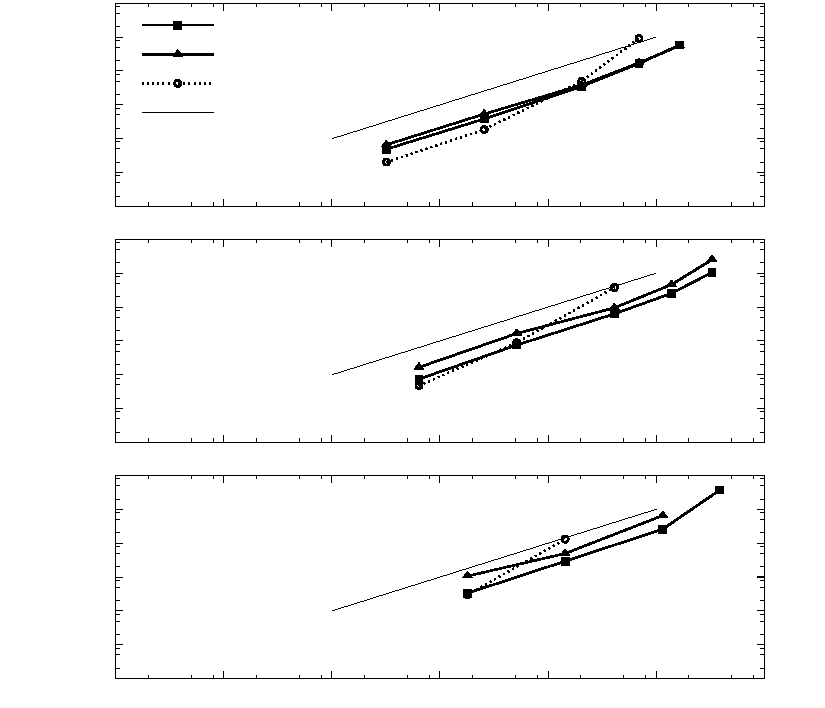
\includegraphics{ConstCoeffPoissonScaling}}%
    \gplfronttext
  \end{picture}%
\endgroup
